% Author @ Sam Appleton, IN_PROGRESS, Reviewer @ Jeremy Perez, Due Date 11/11
\subsection{Strategic Random d-partite Test Generation}
Creating random d-partite graphs with known maximum matching is not trivial work. 
Making a random graph and then running a solver on it is unoptimal, as it requires 
a known, correct solver. Additionally, it takes a non-negligible amount of time to
run on each generated test as $n$ increases.

The difficulty of generating test graphs is that edges have to be chosen strategically 
so that any generated graph has a known maximum matching. Randomness is still a desired 
aspect of test generation so that the testing suite is diverse, but a maximum matching
must still be derived from the created graph. 

An observation on maximum matchings is exploited to create random test graphs 
more efficiently: 
\newtheorem{observation}{Observation}
\begin{observation}
A maximum matching can only ever be as large as the number of vertices
visited in the dimension with the least amount of vertices used by all the hyperedges in 
the graph. A vertex $v$ in a dimension $d$ is defined as `visited' iff $\exists$ a hyperedge $e$
such that $e[d] = v$.
\end{observation}

\begin{figure}[t!]
    \centering
    \begin{minipage}{0.45\textwidth}
        \centering
        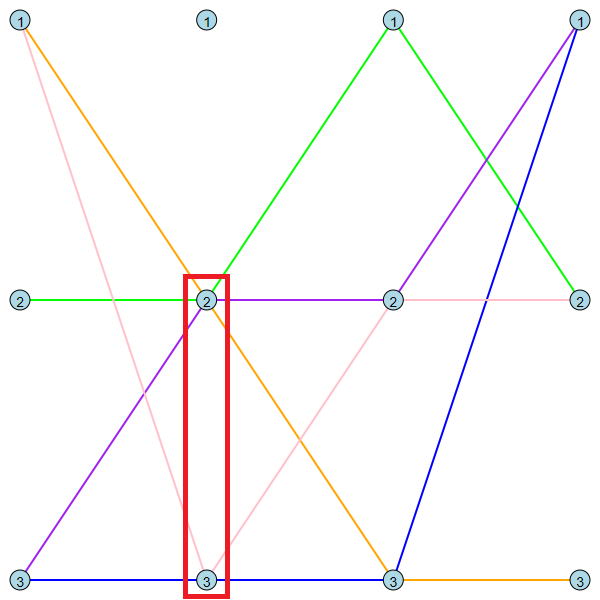
\includegraphics[width=\textwidth]{images/basic.png}
        \caption{An example of the dimension with the least visited vertices. Note that 
        every dimension except the second has an edge that goes through all three vertices.}
        \label{fig:image1}
    \end{minipage}
    \hfill
\end{figure}

This observation derives itself by considering that all hyperedges must pass
through exactly one vertex in each dimension. That means that in any of the dimensions
with the smallest number of visited vertices, at most one edge can be considered for a
maximum matching in vertex. Thus the maximum matching cannot be greater than the
number of vertices in this dimension. 

We exploit this observation to generate a graph with a known matching. To create a 
graph consisting of $d$ dimensions with $n$ vertices, $m$ hyperedges, and a maximum
matching of size $M$, consider the following algorithm:

\begin{algorithmic}
\STATE Create a $d$-partite graph $G$ with dimensions $1, 2, ..., d$ which contain vertices $1, 2, ..., n$.
\FOR{$i$ in $M$}
    \STATE Add a random hyperedge to $G$ such that the hyperedge conflicts on no dimension with any other hyperedge in $G$.
\ENDFOR
\STATE Randomly select an integer $r$ such that $1 \leq r \leq n$. 
\STATE Store the vertex in each hyperedge at index $r$ in list $included$
\FOR{$j$ in $(M - m)$}
    \STATE Add a random hyperedge $e$ such that each of the following is true:
    \begin{itemize}
        \item $e$ is not already a hyperedge in $G$, and
        \item $e[r]$ must be equal to a vertex from $included$.
    \end{itemize}
\ENDFOR
\RETURN $G$
\end{algorithmic}

This algorithm creates a graph with a known dimension with the least visited 
vertices, that being at dimension $r$. Normally this observation only yields an upper-limit 
on a maximum matching as it is not guaranteed that the maximum matching 
necessarily contains an edge for each vertex in the dimension with the least visited 
vertices. However, this algorithm guarantees that a maximum matching does visit 
each vertex, as the edges in the first for loop are guaranteed to be represented in this 
dimension. 

\begin{figure}[t!]
    \centering
    \begin{minipage}{0.95\textwidth}
        \centering
        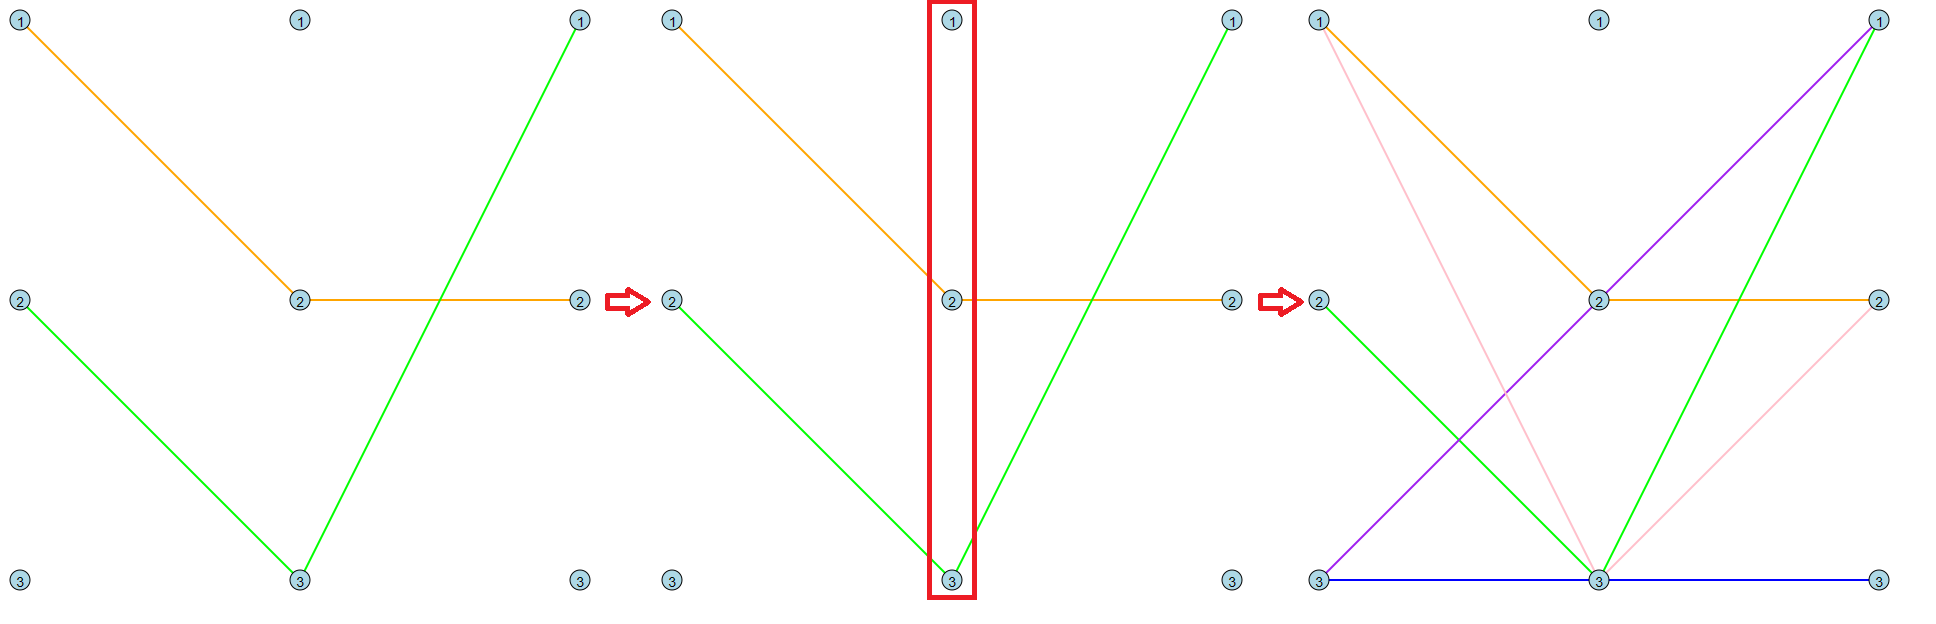
\includegraphics[width=\textwidth]{images/exclude.png}
        \caption{An example of the Dimension Restriction algorithm. In this example, a graph begins with 2 hyper edges on it. $r$ is randomly chosen to be $2$. Then more edges are added that conflict on $2$ or $3$.}
        \label{fig:image1}
    \end{minipage}
    \hfill
\end{figure}

This strategy is not without flaw. Consider a naive algorithm that determines the dimension 
with the least visited vertices and simply returns the number of visited vertices as the
 size of a maximum matching. The tests generated by this algorithm guarantee
 such an algorithm always finds the correct size of the maximum matching, and 
thus is deemed accurate despite not being so. 

A more sophisticated algorithm could be created to solve this weakness. Such an 
algorithm chooses to add hyperedges such that dimension $r$ would not necessarily 
be the dimension with the least visited vertices. To do so, this strategically adds an edge
such that it does not increase the maximum matching, 
but also visits a vertex that no other edge visits. This is done by ensuring the
added edge conflicts with some edge in the known matching on every dimension other than 
$r$, but more research can is required in this regard.